% hello.tex - Our first LaTeX example! This is a comment!

\documentclass{article}
\usepackage{graphicx}
%\usepackage{xunicode} % Unicode support for LaTeX character names (accents, European chars, etc)
\usepackage{xltxtra} % Extra customizations for XeLaTeX

\begin{document}
Hello world!

\textbf{bold!!!}

It does not matter whether you
enter one or several             spaces
after a word.

An empty line starts a new
paragraph.
\\ \\
\# \$ \% \~n \^o \~a

XeLaTeX: á,é,í

This is an % stupid
% Better: instructive <----
example: Supercal%
            ifragilist%
icexpialidocious

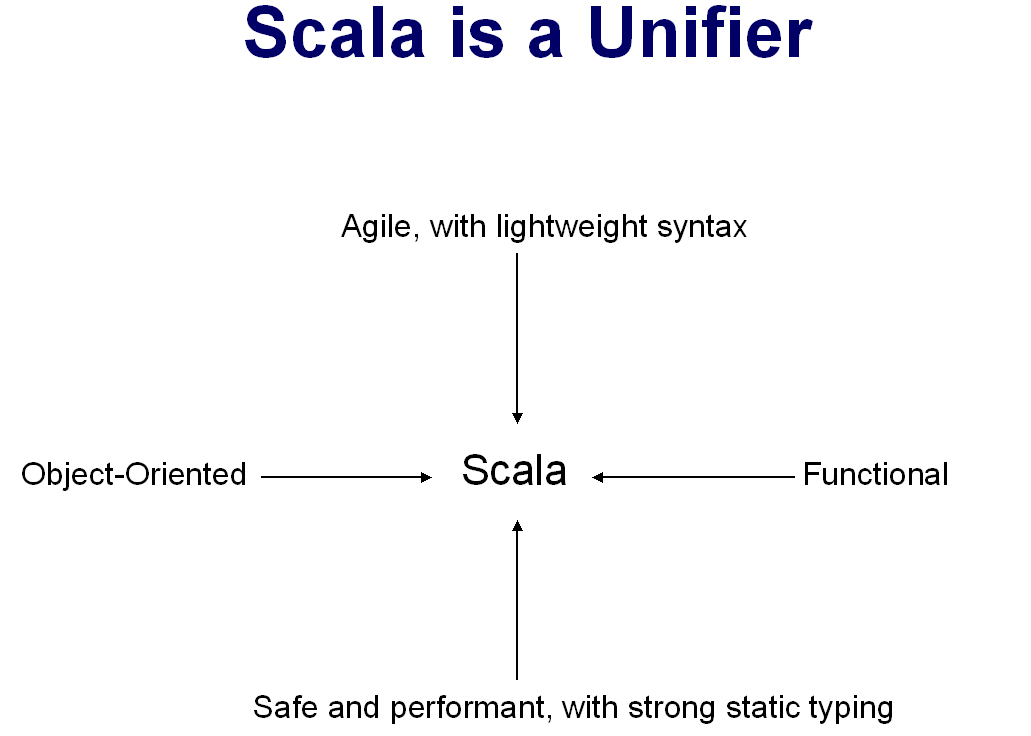
\includegraphics[scale=0.20]{Scala-is-a-Unifier.png}

\end{document}